\documentclass[tikz,border=2pt]{standalone}
\begin{document}
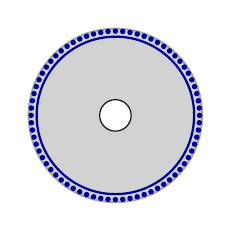
\begin{tikzpicture}
 \fill[gray!35] (0,0) circle (1.1); \draw[gray!70,thick] (0,0) circle (1.1);
 \foreach \i in {0,5,...,355}{\fill[blue!60!black] (\i:1.07) circle (0.035);}
 \draw[blue!60!black,thick] (0,0) circle (1.0);
 \fill[white] (0,0) circle (0.2); \draw (0,0) circle (0.2);
\end{tikzpicture}
\end{document}
